\documentclass{beamer}
\usepackage{graphicx}
\usepackage{graphics}
\usepackage{hyperref}
\usepackage[english]{babel}
\usepackage[T1]{fontenc}
\usepackage[utf8]{inputenc}
\usepackage{xfrac}
\usepackage{array}
\usepackage{multirow}


\mode<presentation>
{
    \usetheme{AMUFree-kk}
    \setbeamercovered{transparent = 28}
}
\title{Zero-shot learning}
\date{2021}
\author{Karol Kaczmarek}
\setbeamertemplate{bibliography item}{[\theenumiv]}


\begin{document}

\begin{frame}
    \titlepage
\end{frame}

\iffalse
\AtBeginSection[]
{
    \begin{frame}
        \frametitle{Outline}
        \tableofcontents[currentsection]
    \end{frame}
}
\fi

% Pretrain-finetune
\begin{frame}
    \frametitle{Pretrain-finetune}
    \begin{center}
        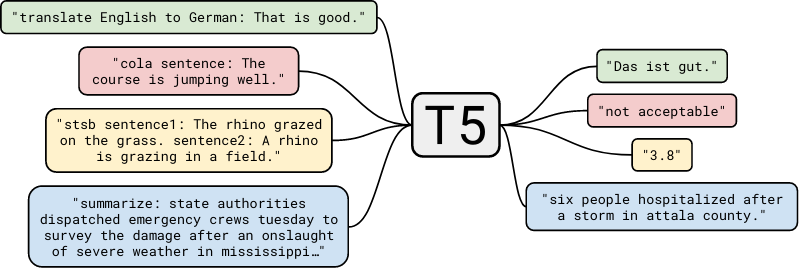
\includegraphics[scale=1.1]{img/t5.png}
    \end{center}
    \begin{itemize}
        \item Standard procedure: pretrain-finetune: BERT \cite{bert}, RoBERTa \cite{roberta}, T5 \cite{t5}, ...
        \begin{itemize}
            \item pretrain on huge text or use pretrained model
            \item finetune and evaluate on desired task
        \end{itemize}
    \end{itemize}
    \begin{center}
        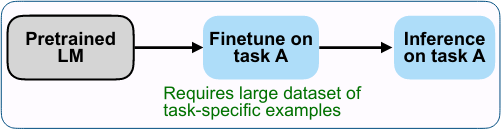
\includegraphics[scale=1.5]{img/zero_shot_method0.png}
    \end{center}
\end{frame}


% Prompting
\begin{frame}
    \frametitle{Prompting \cite{scale_prefix_tuning}}
    \begin{center}
        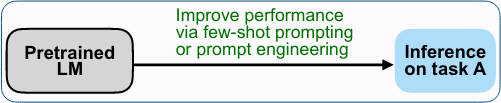
\includegraphics[scale=1.5]{img/zero_shot_method1.png}
    \end{center}
    \begin{center}
        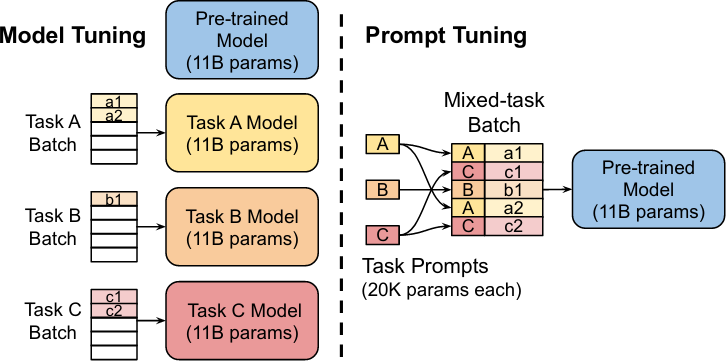
\includegraphics[scale=1.3]{img/tuning_vs_prompt.png}
    \end{center}
\end{frame}

\begin{frame}
    \frametitle{Prompting \cite{prefix_tuning}}
    \begin{center}
        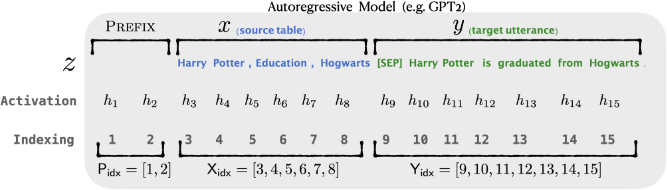
\includegraphics[scale=1.7]{img/prefix_models_decoder.png}
    \end{center}
    \begin{center}
        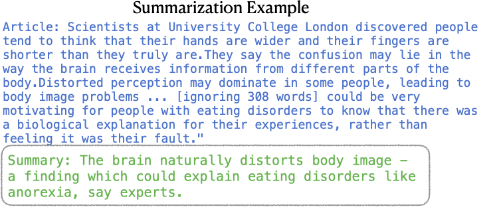
\includegraphics[scale=1.5]{img/prefix_models_decoder_example.png}
    \end{center}
\end{frame}

\begin{frame}
    \frametitle{Prompting \cite{prefix_tuning}}
    \begin{center}
        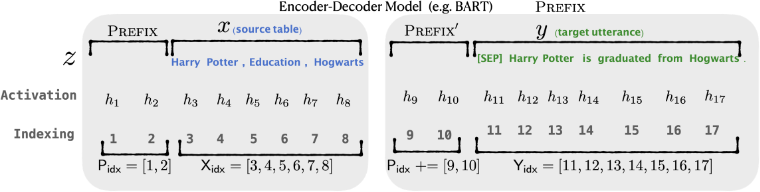
\includegraphics[scale=1.7]{img/prefix_models_encoder_decoder.png}
    \end{center}
    \begin{center}
        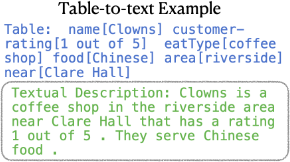
\includegraphics[scale=1.5]{img/prefix_models_encoder_decoder_example.png}
    \end{center}
\end{frame}

\begin{frame}
    \frametitle{Prompting - GPT-3 \cite{gpt3}}
    \begin{center}
        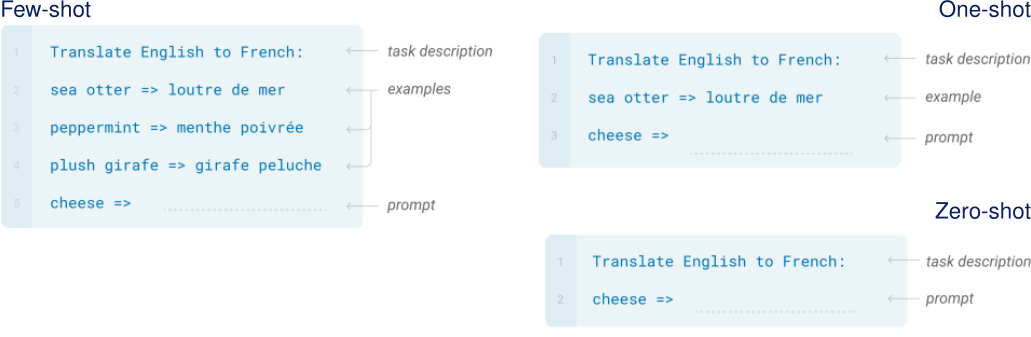
\includegraphics[scale=1.35]{img/gpt3_all_shot.png}
    \end{center}
\end{frame}


% Instruction training
\begin{frame}
    \frametitle{FLAN}
    \begin{itemize}
        \item September 2021, Google
        \item FLAN (\textbf{F}inetuned \textbf{LA}nguage \textbf{N}et) \cite{flan}
        \item 137B parameter pretrained language model (like GPT-3)
        \item Improving zero-shot learning on over 60 NLP tasks
        \item \textbf{Instruction tuning} - verbalize NLP tasks by natural language instruction templates
    \end{itemize}
\end{frame}

\begin{frame}
    \frametitle{Instruction training}
    \begin{center}
        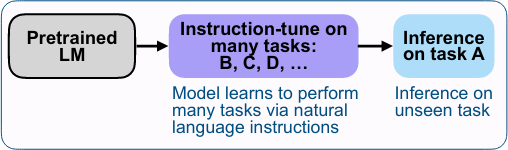
\includegraphics[scale=1.4]{img/zero_shot_method2.png}
    \end{center}
    \begin{itemize}
        \item \footnotesize{teach language model to perform tasks described via \textbf{instructions}, it will \textbf{learn to follow instructions} and do so even for unseen tasks}
        \item \footnotesize{group tasks into \textbf{clusters by task type} and hold out each task cluster for evaluation while instruction tuning on all remaining clusters}
        \item Intuition - \footnotesize{NLP tasks can be described:}
        \begin{itemize}
            \item \footnotesize{"Is the sentiment of this movie review positive or negative?"}
            \item \footnotesize{"Translate ‘how are you’ into Chinese."}
        \end{itemize}          
    \end{itemize}
\end{frame}

\begin{frame}
    \frametitle{Instruction training}
    \begin{center}
        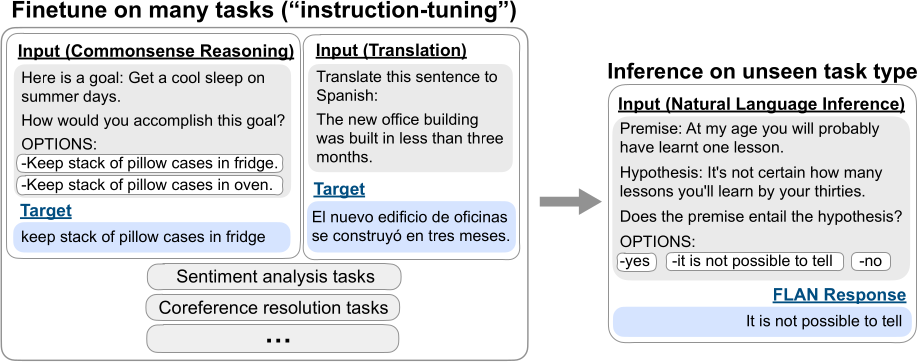
\includegraphics[scale=1.4]{img/instruction_tuning.png}
    \end{center}
    \begin{itemize}
        \item \footnotesize{(!!!) include \textbf{OPTIONS} to makes the model aware of which choices are desired when responding}
    \end{itemize}
\end{frame}

\begin{frame}
    \frametitle{Cluster templates}
    \begin{center}
        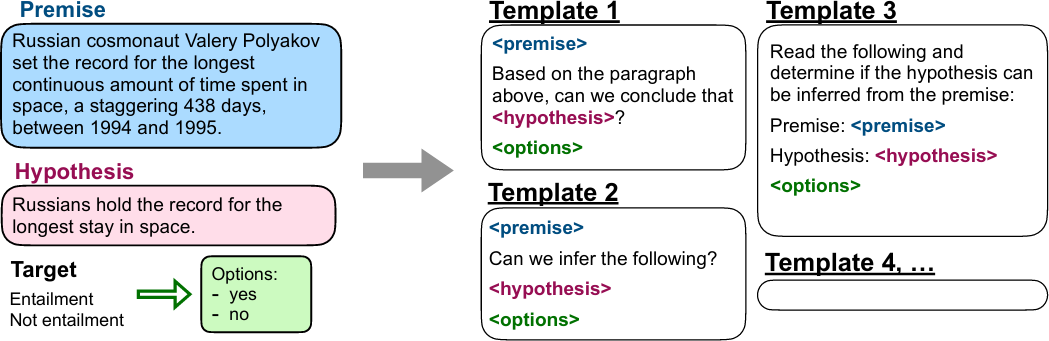
\includegraphics[scale=1.2]{img/templates.png}
    \end{center}
    \begin{itemize}
    \footnotesize
        \item manually compose \textbf{10 unique templates} that describe the task using natural language instructions (10 templates per task)
        \item include up to \textbf{3 templates} that "turned the task around" (generate negative movie review for sentiment classification)
        \item \textbf{randomly selected} instruction template for tasks in pretraining
    \end{itemize}
\end{frame}

\begin{frame}
    \frametitle{Task clusters}
    \begin{center}
        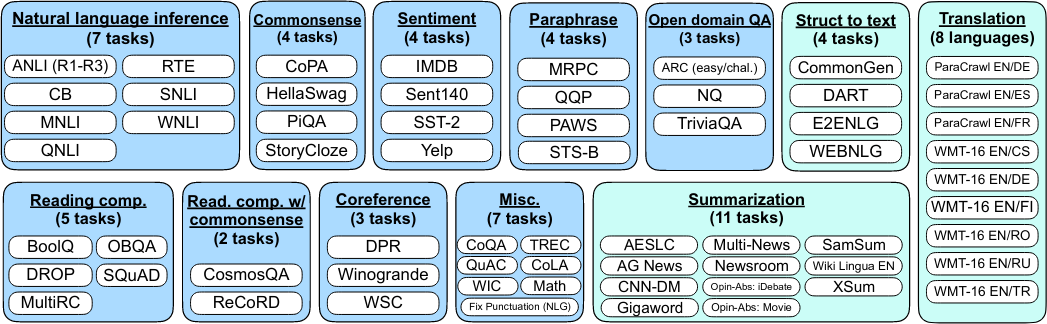
\includegraphics[scale=1.2]{img/task_clusters.png}
    \end{center}
    \begin{itemize}
    \footnotesize
        \item aggregate \textbf{62 text datasets} (including both language understanding and language generation tasks) into a single mixture
        \item each dataset is \textbf{categorized into one of twelve} task clusters (given cluster are of the same task type)
        \item evaluate on cluster that \textbf{were not} during instruction tuning
    \end{itemize}
\end{frame}

\begin{frame}
    \frametitle{Task clusters}
    \begin{center}
        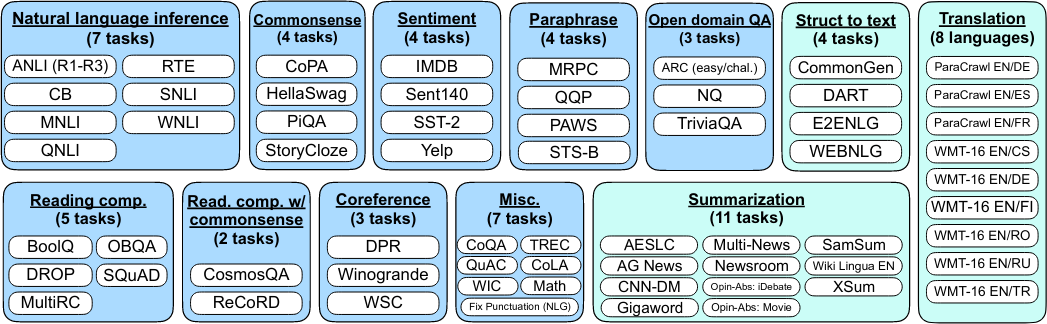
\includegraphics[scale=1.2]{img/task_clusters.png}
    \end{center}
    \begin{itemize}
        \item \footnotesize{some datasets have more than ten million training examples (translation) - limit the number of training examples per dataset to \textbf{30000}}
        \item \footnotesize{other datasets have few training examples (CommitmentBank only has \textbf{250}) - use \textbf{examples-proportional mixing} scheme (from T5 - probability of example sampling) to prevent datasets from being marginalized}
    \end{itemize}
\end{frame}

\begin{frame}
    \frametitle{Task clusters}
    \begin{itemize}
    \footnotesize
        \item \textbf{Natural language inference (NLI)} concerns how two sentences relate, typically asking, given a first sentence, whether a second sentence is true, false, or possibly true
        \item \textbf{Reading comprehension} tests the ability to answer a question when given a passage that contains the answer
        \item \textbf{Open-domain QA} asks models to answer questions about the world without specific access to information that contains the answer
        \item \textbf{Commonsense reasoning} evaluates the ability to perform physical or scientific reasoning with an element of common sense
        \item \textbf{Coreference resolution} tests the ability to identify expressions of the same entity in some given text
        \item \textbf{Translation} is the task of translating text from one language into a different language
    \end{itemize}
\end{frame}

\begin{frame}
    \frametitle{Architecture}
    \begin{itemize}
        \item \textbf{left-to-right}, \textbf{decoder-only} transformer language model of \textbf{137B parameters}
        \begin{itemize}
            \item model from Google publication - generate computer programs in a programming language (program synthesis)
        \end{itemize}
        \item pretrained on a collection of web documents (including
those with \textbf{computer code}), \textbf{dialog data}, and \textbf{Wikipedia} - dataset \textbf{is not as clean} as the GPT-3 training set and also \textbf{has a mixture of dialog and code}
        \item used models:
        \begin{itemize}
            \item \textbf{Base LM} - pretrained model that was used for program synthesis
            \item \textbf{FLAN} - instruction-tuned version of \textbf{Base LM}
        \end{itemize}
    \end{itemize}
\end{frame}

\begin{frame}
    \frametitle{Score}
    \begin{center}
        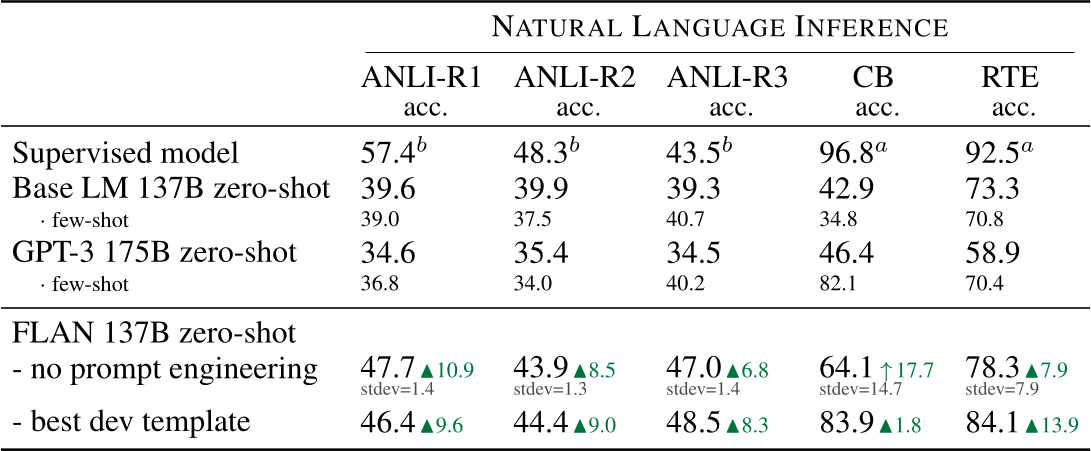
\includegraphics[scale=1.05]{img/score_nli.png}
    \end{center}
    \tiny{$^a$T5-11B, $^b$BERT-large, 
\includegraphics[scale=1.0]{img/up_arrow_1.png} improvement over few-shot GPT-3, 
\includegraphics[scale=1.0]{img/up_arrow_2.png} improvement only over zero-shot GPT-3}
    \begin{itemize}
    \footnotesize
        \item using the same prompts as GPT-3 for \textbf{zero} and \textbf{few-shot} Base LM results
        \item NLI examples are unlikely to have appeared naturally in an training set
        \item FLAN question: "Does <premise> mean that <hypothesis>?"
    \end{itemize}
\end{frame}

\begin{frame}
    \frametitle{Score}
    \begin{center}
        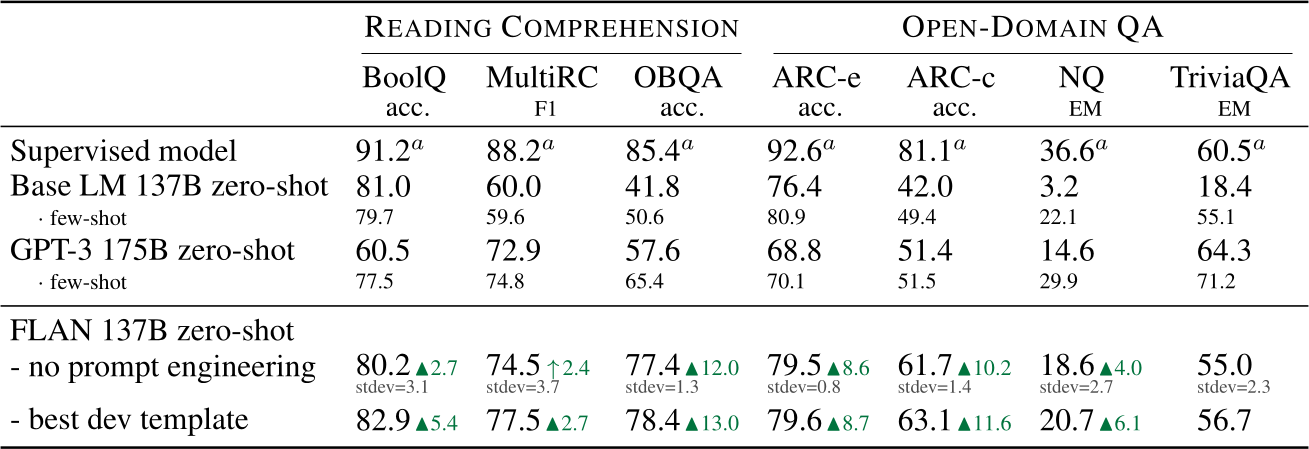
\includegraphics[scale=1.0]{img/score_rc_qa.png}
    \end{center}
    \tiny{$^a$T5-11B, 
\includegraphics[scale=1.0]{img/up_arrow_1.png} improvement over few-shot GPT-3, 
\includegraphics[scale=1.0]{img/up_arrow_2.png} improvement only over zero-shot GPT-3}
    \begin{itemize}
    \footnotesize 
        \item \textbf{reading comprehension} is where models are asked to answer a question about a provided passage
    \end{itemize}
\end{frame}

\begin{frame}
    \frametitle{Score}
    \begin{center}
        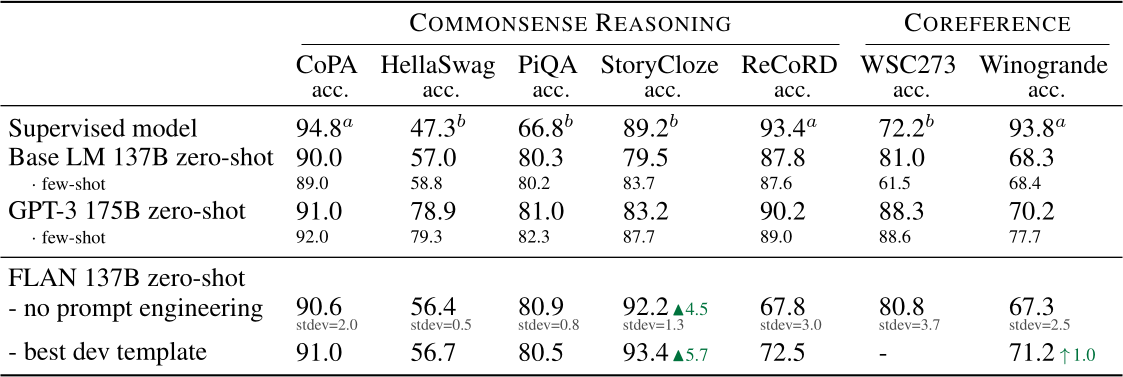
\includegraphics[scale=1.15]{img/score_cr_c.png}
    \end{center}
    \tiny{$^a$T5-11B, $^b$BERT-large, 
\includegraphics[scale=1.0]{img/up_arrow_1.png} improvement over few-shot GPT-3, 
\includegraphics[scale=1.0]{img/up_arrow_2.png} improvement only over zero-shot GPT-3}
    \begin{itemize}
    \footnotesize 
        \item \textbf{Commonsense reasoning} evaluates the ability to perform physical or scientific reasoning with an element of common sense
        \item \textbf{Coreference resolution} tests the ability to identify expressions of the same entity in some given text
        \item Model fails when instructions are not crucial for describing task
    \end{itemize}
\end{frame}

\begin{frame}
    \frametitle{Score}
    \begin{center}
        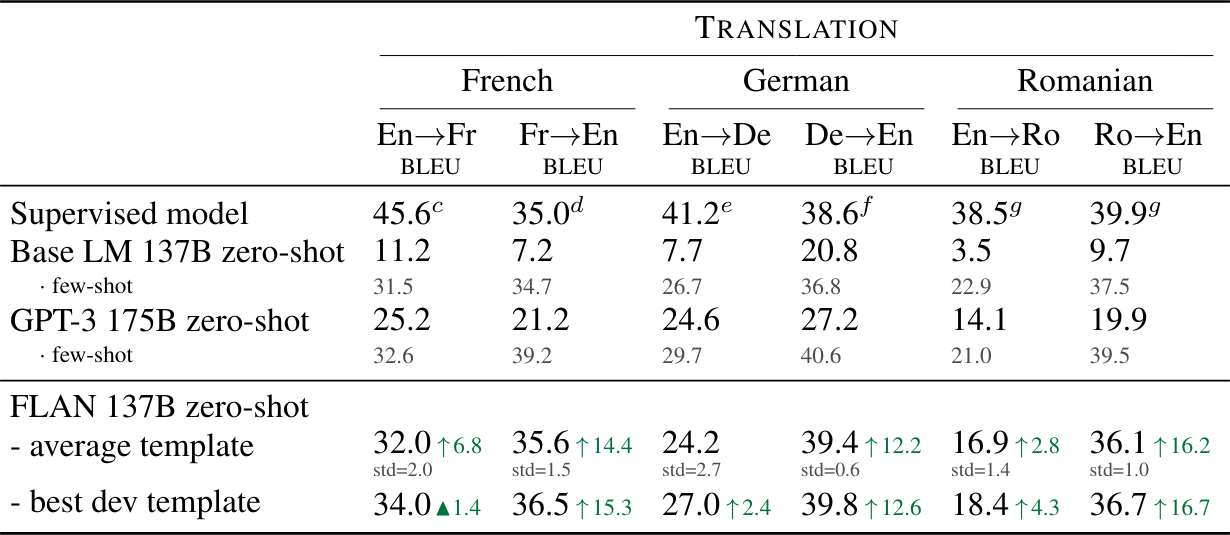
\includegraphics[scale=1.05]{img/score_translation.png}
    \end{center}
    \tiny{
\includegraphics[scale=1.0]{img/up_arrow_1.png} improvement over few-shot GPT-3, 
\includegraphics[scale=1.0]{img/up_arrow_2.png} improvement only over zero-shot GPT-3}
    \begin{itemize}
    \footnotesize 
        \item GPT-3: $\sim$7\% of text in other language ($\sim$1,5 fr, $\sim$1,5 de)
        \item FLAN: $\sim$10\% of text in other language
    \end{itemize}
\end{frame}

\begin{frame}
    \frametitle{Instruction tuning}
    \begin{itemize}
        \item is \textbf{very effective} on tasks that \textbf{can be naturally verbalized} as instructions (natural language inference and question answering)
        \item is \textbf{less effective} on tasks that are \textbf{directly formulated} as language modeling (commonsense reasoning and coreference resolution)
    \end{itemize}
\end{frame}

\begin{frame}
    \frametitle{Clusters used for instruction tuning}
    \begin{center}
        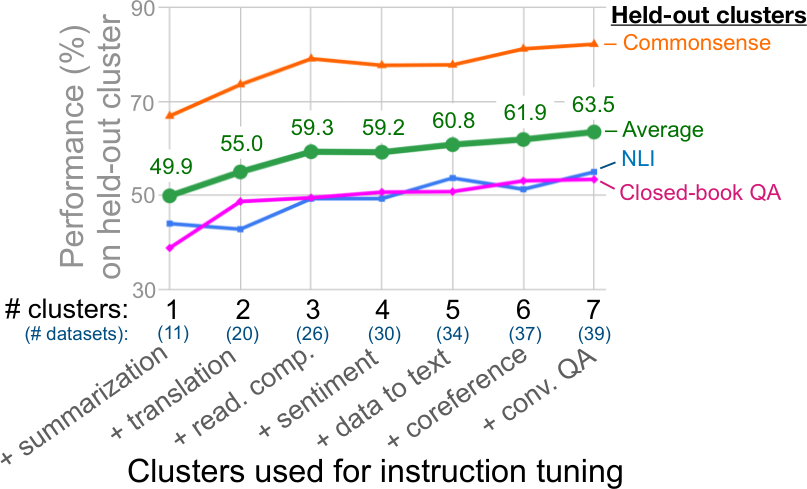
\includegraphics[scale=1.35]{img/score_instruction_tuning.png}
    \end{center}
    \footnotesize Increasing the number of task clusters improves perform.
\end{frame}

\begin{frame}
    \frametitle{Instruction tuning - performance on \textbf{seen} tasks}
    \begin{center}
        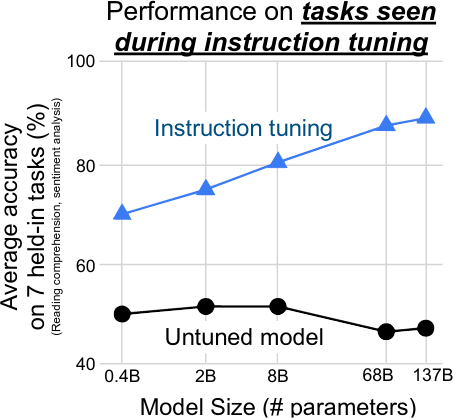
\includegraphics[scale=1.6]{img/performance_1.png}
    \end{center}
    \footnotesize Untuned model - untuned model without instruction tuning
\end{frame}

\begin{frame}
    \frametitle{Instruction tuning - performance on \textbf{unseen} tasks}
    \begin{center}
        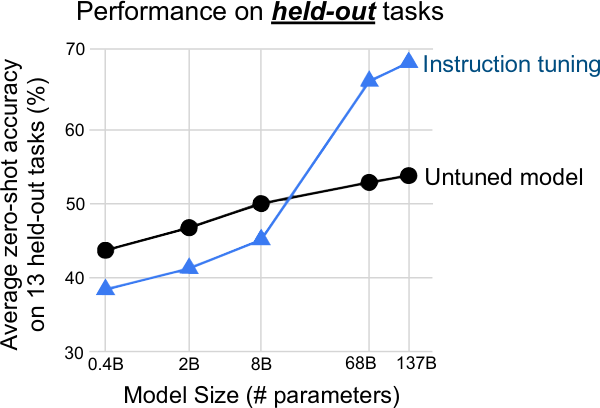
\includegraphics[scale=1.5]{img/performance_2.png}
    \end{center}
    \footnotesize Hurts performance on 8B and smaller models - learning the $\sim$40 tasks \textbf{fills the entire model capacity}, causing these models to perform worse on new tasks
\end{frame}

\begin{frame}
    \frametitle{Prompt tuning - SuperGLUE}
    \begin{center}
        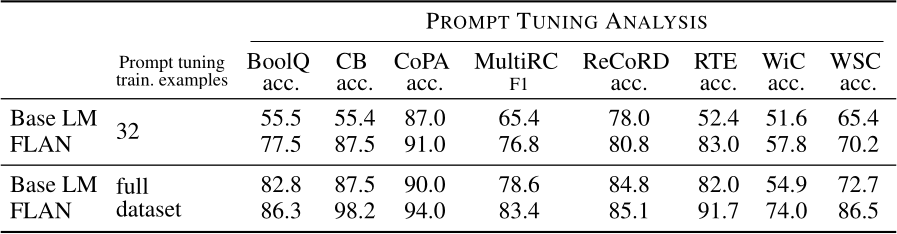
\includegraphics[scale=1.5]{img/prompting_analysis.png}
    \end{center}
    \footnotesize FLAN \textbf{responds better} to continuous inputs attained via prompt tuning than Base LM. When prompt tuning on a given dataset, \textbf{no tasks from the same cluster} as that dataset were seen during instruction tuning
\end{frame}

\begin{frame}
    \frametitle{Few-shot}
    \begin{center}
        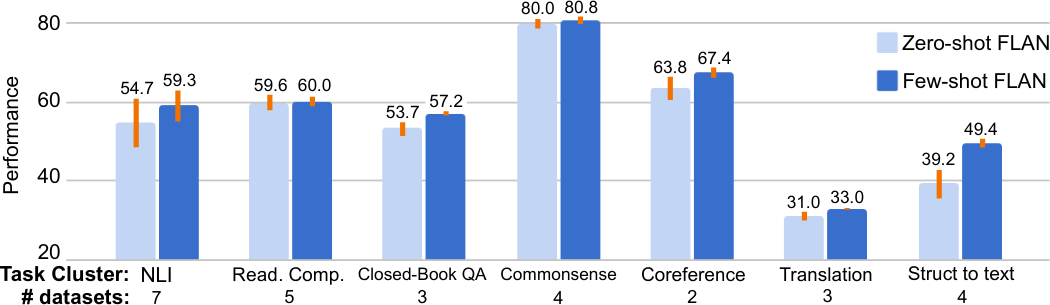
\includegraphics[scale=1.25]{img/performance_final.png}
    \end{center}
    \footnotesize Standard deviation (orange color) among templates is \textbf{lower} for few-shot FLAN, indicating reduced sensitivity to prompt engineering.
\end{frame}

\begin{frame}
    \frametitle{Environmental consideration}
    \begin{itemize}
        \item energy cost and carbon footprint for the pretrained models were \textbf{451 MWh} and \textbf{26 tCO2e}
        \item additional instruction tuning gradient-steps for finetuning FLAN is \textbf{less than 2\%} of the number of pretraining steps
    \end{itemize}
\end{frame}


% References
\section{References}
\begin{frame}[allowframebreaks,t]
    \tiny
    \frametitle{References}
    \bibliographystyle{ieeetr}
    \bibliography{zero_shot}
    %\nocite{*}
\end{frame}

\end{document}
